% STScI Poster Aug 27, 2020
% Nathaniel Starkman


%%%%%%%%%%%%%%%%%%%%%%%%%%%%%%%%%%%%%%%%%
% Beamer Presentation
% LaTeX Template
% Version 1.0 (10/11/12)
%
% This template has been downloaded from:
% http://www.LaTeXTemplates.com
%
% License:
% CC BY-NC-SA 3.0 (http://creativecommons.org/licenses/by-nc-sa/3.0/)
%
% Gemini theme
% https://github.com/anishathalye/gemini
%
%%%%%%%%%%%%%%%%%%%%%%%%%%%%%%%%%%%%%%%%%


\documentclass[final]{beamer}

% ====================
% Packages
% ====================

\usepackage[T1]{fontenc}
\usepackage{lmodern}
\usepackage[size=custom,width=120,height=72,scale=1.1]{beamerposter}
\usetheme{gemini}
\usecolortheme{gemini}
\usepackage{graphicx}
\usepackage{booktabs}
\usepackage{tikz}
\usepackage{pgfplots}
\usepackage{subfig}

% ====================
% Lengths
% ====================

% If you have N columns, choose \sepwidth and \colwidth such that
% (N+1)*\sepwidth + N*\colwidth = \paperwidth
\newlength{\sepwidth}
\newlength{\colwidth}
\setlength{\sepwidth}{0.025\paperwidth}
\setlength{\colwidth}{0.3\paperwidth}

\newcommand{\separatorcolumn}{\begin{column}{\sepwidth}\end{column}}

% ====================
% Title
% ====================

\title{Stellar Stream Track Reconstruction, with Errors}

\author{Nathaniel Starkman \inst{1} \and Daniela Calvetti \& Erkki Somersalo \inst{2} \and Jeremy Webb \inst{1} \and Jo Bovy \inst{1}}

\institute[shortinst]{\inst{1} Astronomy and Astrophysics, University of Toronto \samelineand \inst{2} Department of Mathematics, Case Western Reserve University}

\setbeamertemplate{headline}
{
  \begin{beamercolorbox}{headline}
    \begin{columns}
        \begin{column}{0.25\paperwidth}
            \centering
            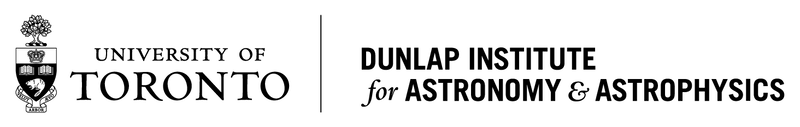
\includegraphics{figures/logos/Dunlap_CombinationIdentityUofT_Eng_Black.png}
        \end{column}
        \begin{column}{0.5\paperwidth}
            \usebeamerfont{headline}
            \vskip3ex
            % \centering
            {\usebeamerfont{headline title}\usebeamercolor[fg]{headline title}\inserttitle\\[0.5ex]}
            {\usebeamerfont{headline author}\usebeamercolor[fg]{headline author}\insertauthor\\[1ex]}
            {\usebeamerfont{headline institute}\usebeamercolor[fg]{headline institute}\insertinstitute\\[1ex]}
        \end{column}
        \begin{column}{0.25\paperwidth}
            \centering
            
\includegraphics{figures/logos/cwru-formal-logo-blue-no-tag.png}
        \end{column}
    \end{columns}
    \vspace{5ex}
    \ifbeamercolorempty[bg]{headline rule}{}{
      \begin{beamercolorbox}[wd=\paperwidth,colsep=0.5ex]{headline rule}\end{beamercolorbox}
    }
  \end{beamercolorbox}
}


% ====================
% Body
% ====================

\begin{document}

\begin{frame}[t]
\begin{columns}[t]
\separatorcolumn

\begin{column}{\colwidth}

    \begin{alertblock}{Introduction}

        Stellar streams are sensitive probes of the Galactic potential. The likelihood of a model given stream data can only be assessed using simulations. However, comparison to simulation is challenging in a noisy 6D phase space in which even the stream paths are hard to quantify. Here we present a novel application of Self-Organizing Maps and first-order Kalman Filters to  reconstruct the stream path, propagating measurement errors and data sparsity into the stream path uncertainty. The technique is Galactic-model independent, non-parametric, and works on phase-wrapped streams. We can uniformly analyze and compare data with simulation.

    \end{alertblock}

    \begin{block}{Data Ordering}

        Using Self-Organizing Maps (SOM) pre-trained on locally linearizing reference frames, we discover the 1D structure of a stellar stream and a path-distance-minimizing data ordering.

        \heading{Self-Organizing Maps (SOM)}

            SOM are a neural network for low-dimensional, discrete representation of data.  Using linked prototype vectors, SOM approximate the data by iteratively updating the topology of the prototypes to approximate the data distribution. In final form, each prototype maps nearby high-dimensional data to a lower-dimensional lattice \cite{9780387733937} -- see Fig. \ref{fig:data_ordering}.

        \heading{Linearizing Reference Frames}

            Streams orbit the Galactic center of mass. The orbit path for the majority of streams, distant and less sensitive to Galactic structure, approximately describe a great circle. 
            
            Therefore, for a fixed origin point ($\alpha^*, \delta$), and rotation $\theta$ the transformation
            to a great circle frame
            % \begin{equation}
            %     R = \left[\begin{matrix}
            %             1 &   &   \\
            %               & - \cos{\left(\theta \right)} & \sin{\left(\theta \right)} \\
            %               & - \sin{\left(\theta \right)} & \cos{\left(\theta \right)}
            %     \end{matrix}\right]
            %     \cdot
            %     \left[\begin{matrix}
            %             - \cos{\left(\delta \right)} &   & - \sin{\left(\delta \right)} \\
            %               & 1 &   \\
            %             \sin{\left(\delta \right)} &   & - \cos{\left(\delta \right)}
            %     \end{matrix}\right]
            %     \cdot
            %     \left[\begin{matrix}
            %         \cos{\left(\alpha \right)} & - \sin{\left(\alpha \right)} &   \\
            %         \sin{\left(\alpha \right)} & \cos{\left(\alpha \right)} &   \\
            %           &   & 1
            %     \end{matrix}\right]
            % \end{equation}
            defines a locally-linearizing set of sky coordinates ($\phi_1, \phi_2$) \cite{jobovy/stellarkinematics}. By ordering data along $\phi_1$ we discover the approximate data ordering and circumvent the SOM network burn-in phase.
    
            \begin{figure}
                \centering
                \captionsetup{justification=centering}
                \caption{\textbf{\normalsize{Mock Stellar Stream at Solar Circle.}
                         \newline
                         Data coloring is index order.
                         Errors are ${\sim2}\times$ standard for cold streams.}
                         \label{fig:data_ordering}}
                \subfloat[ \textbf{Mock Stream, randomly ordered.} ]{ 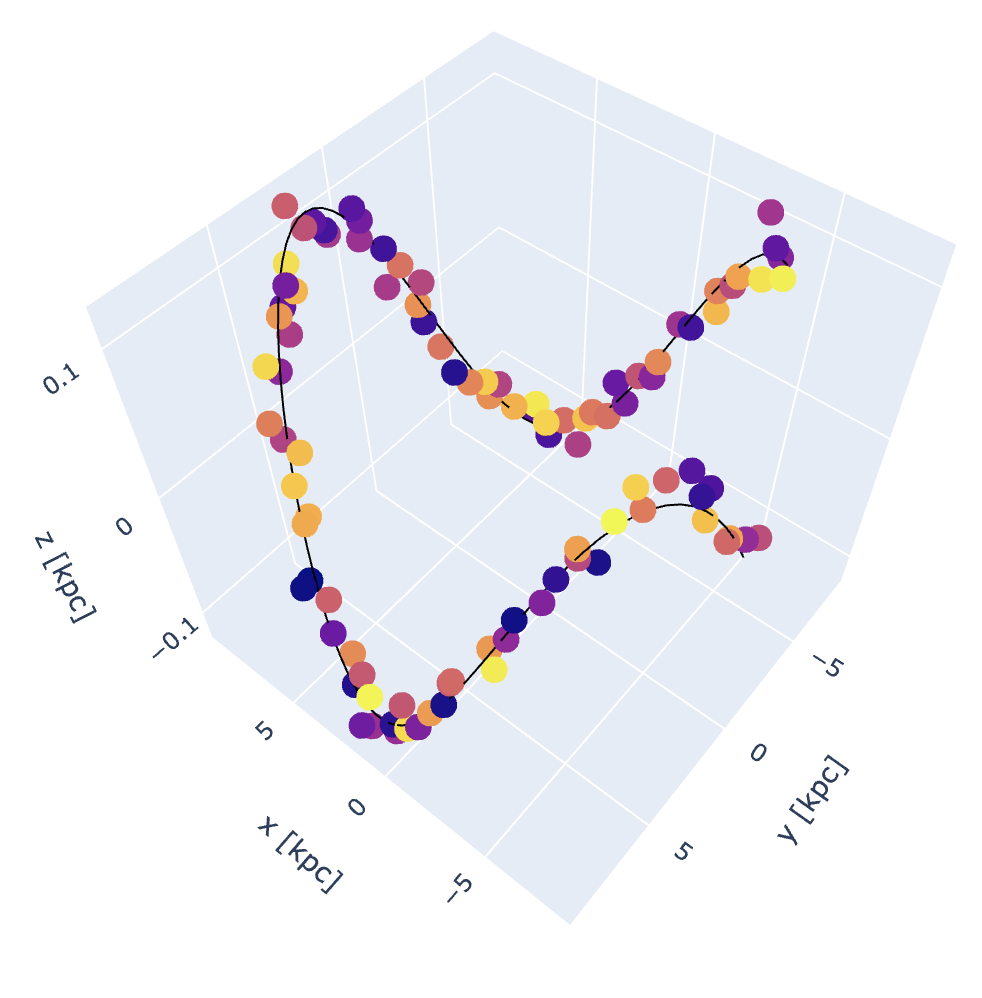
\includegraphics[width=0.4\linewidth]{figures/solar_circle_stream.png} }%
                \quad
                \subfloat[ \textbf{Projection, reindexing by SOM} ]{ 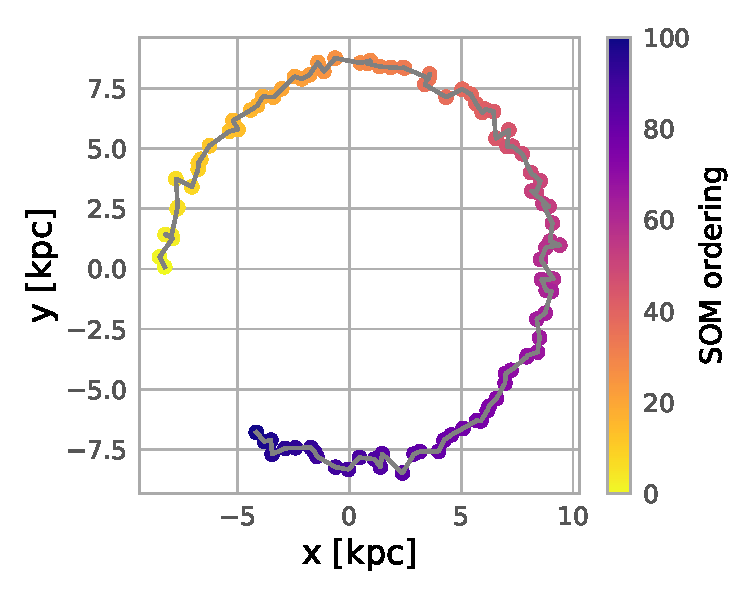
\includegraphics[width=0.5\linewidth]{figures/SOM_ordering.pdf} }%
            \end{figure}

    \end{block}


\end{column}

\separatorcolumn

\begin{column}{\colwidth}

    \begin{block}{Reconstructing Stream Paths}

        \textbf{A first-order Newtonian-dynamics, hidden-variable Kalman Filter is used to construct the stream path, propagating both measurement and sampling-sparsity-induced uncertainty into the path. The technique is injective and produces its own affine parameterization.}

        \begin{figure}
            \centering
            \caption{\normalsize{\textbf{Reconstructed Stream Path \& Uncertainties (blue).}} \label{fig:kalman_path}\vspace{-30pt}}
            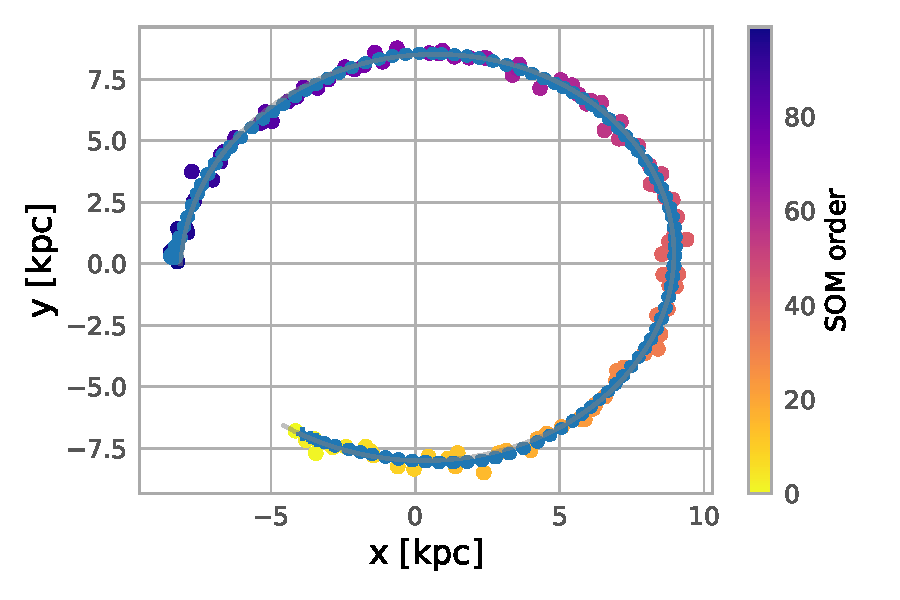
\includegraphics[width=1.05\linewidth]{figures/kalman_path_xy.pdf}
        \end{figure}

        \vspace{-45pt}

        \begin{figure}
            \centering
            \caption{\normalsize{\textbf{Path Residual: uncertainties reflect data.}\label{fig:path_residual}} \vspace{-60pt}}
            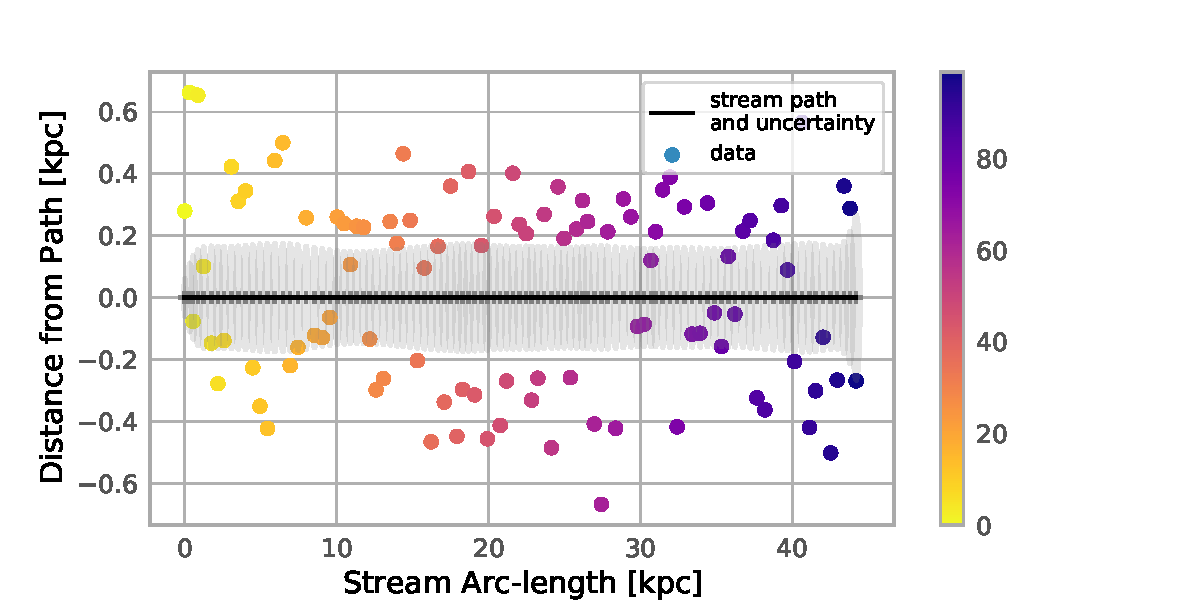
\includegraphics[width=1.2\linewidth]{figures/path_residual.pdf}
        \end{figure}

        % To use Kalman filter techniques we interpret the SOM data ordering as a time-series in which the time intervals are unknown. As proxy we tune each time step by the window-averaged point-to-point distance, such that time steps track local density.
        % \begin{figure}
        %     \centering
        %     \caption{\normalsize{\textbf{Tuning Distance Steps over SOM index.}}\label{fig:time_proxy}\vspace{-30pt}}
        %     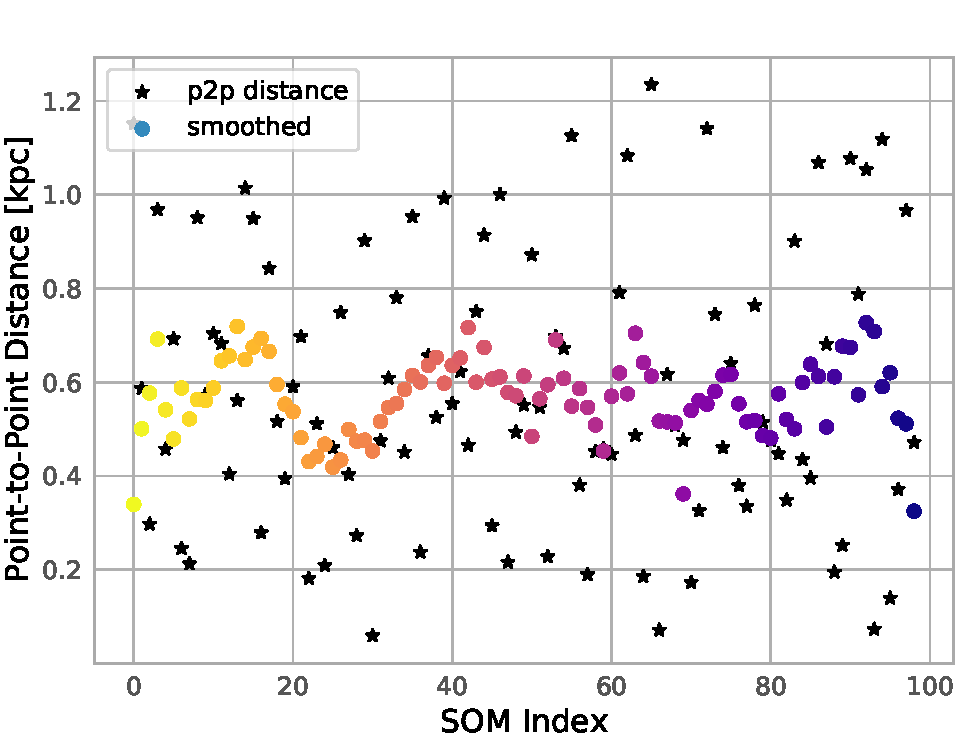
\includegraphics[width=0.45\linewidth]{figures/time_proxy.pdf}
        % \end{figure}


    \end{block}

\end{column}

\separatorcolumn

\begin{column}{\colwidth}

    \begin{block}{Kalman Filter Math}

            Kalman filters estimate a joint probability distribution over the variables in a timeseries. For a hidden-velocity filter the state vector $\hat{\mathbf{x}}$ encodes the position and pseudo-velocity, and $\mathbf{P}$ the error therein. The Newtonian-dynamics transition matrix $\mathbf{F}$ gives the (prior) dynamics between states and $\mathbf{Q}$ the associated uncertainty, like intrinsic dispersion (see Fig. \ref{fig:path_residual}). $\mathbf{H}$ is the observation function, bringing states into measurement space. $\mathbf{z}$, $\mathbf{R}$ are the measurement mean and noise covariance \cite{KalmanFiltersinPythonby}.
            \begin{equation}
                \hat{\mathbf{x}} = \left[\begin{matrix}
                        x & v_x & y & v_y & z & v_z  \\
                    \end{matrix}\right]^{T}
                \qquad
                \mathbf{F} = \rm{diag}_3 \left(
                    \left[\begin{matrix}
                        1 & \Delta t  \\
                          & 1 \\
                    \end{matrix}\right]
                \right) 
                \qquad
                \mathbf{H} = \left[\begin{matrix}
                        1 & 0 &   &   &   &   \\
                          &   & 1 & 0 &   &   \\
                          &   &   &   & 1 & 0 \\
                    \end{matrix}\right]
            \end{equation}

            The Kalman Filter operates by updating at each time step ($\Delta t$); however, the times are not known. As a proxy, before each predict-update iteration we tune the time-step in the state transition matrix $\mathbf{F}$ by the smoothed point-to-point distance.

            For each data point the Kalman filter process is two steps \cite{9780387733937,KalmanFiltersinPythonby}:
            \begin{flalign}
                \intertext{\hspace{.5\linewidth} \textbf{Predict}}
                %
                \hat{\mathbf{x}}_{k\mid k-1} &= \mathbf F_k\hat{\mathbf{x}}_{k-1\mid k-1} + \mathbf B_k \mathbf u_k  & \text{\textit{a priori} state estimate} \\
                %
                \mathbf{P}_{k\mid k-1} &=  \mathbf F_k \mathbf{P}_{k-1\mid k-1} \mathbf F_k^\mathsf T + \mathbf Q_k & \text{\textit{a priori} estimate covariance} \\
                %
                \intertext{\hspace{.5\linewidth} \textbf{Update}}
                %
                \tilde{\mathbf y}_k &= \mathbf z_k - \mathbf{H}_k\hat{\mathbf{x}}_{k\mid k-1} & \text{pre-fit residual} \\
                %
                \mathbf{S}_k &= \mathbf{H}_k \mathbf{P}_{k\mid k-1} \mathbf{H}_k^\mathsf T + \mathbf{R}_k & \text{pre-fit residual covariance} \\
                %
                \mathbf{K}_k &= \mathbf{P}_{k\mid k-1}\mathbf{H}_k^\mathsf T \mathbf{S}_k^{-1} & \text{optimal Kalman gain} \\
                %
                \hat{\mathbf{x}}_{k\mid k} &= \hat{\mathbf{x}}_{k\mid k-1} + \mathbf{K}_k\tilde{\mathbf y}_k & \text{\textit{a posteriori} estimate} \\
                %
                \mathbf{P}_{k|k} &= (\mathbf{I} - \mathbf{K}_k \mathbf{H}_k) \mathbf{P}_{k|k-1} & \text{\textit{a posteriori} estimate covariance}
            \end{flalign}

            Subsequent steps are updated by previous steps, but not vice versa. To back-propagate information, the process is run in reverse by Rauch–Tung–Striebel (RTS) smoothing \cite{doi:10.2514/3.3166}.
            

    \end{block}

    \begin{alertblock}{Conclusions}

        We reconstruct the mean path of stellar streams (eg Fig. \ref{fig:kalman_path}) from sparse and noisy data, respecting both as sources of error. By using linearizing reference-frame transformations in conjunction with Self-Organizing Maps, we treat stellar-stream data as a pseudo time-series, to which first-order Kalman Filters can be applied. The path reconstruction properly propagates measurement errors and data sparsity into a path error (Fig. \ref{fig:path_residual}), allowing for equal treatment and more precise comparison of data and simulation.

    \end{alertblock}

    \begin{block}{References}
        \vspace{-30pt}
        % \nocite{*}
        \footnotesize{
        \bibliographystyle{plain}
        \bibliography{starkman_stsci_poster}
        }

    \end{block}

\end{column}

\separatorcolumn
\end{columns}
\end{frame}

\end{document}
